

\begin{abstract}[\hspace*{-10pt}]
    This appendix is a postprint of the published work: \fullcite{van_biesbroeck_influence_2023}  % Ce chapitre reprend principalement les travaux publiés dans: 
\end{abstract}

\begin{abstract}
    abstract
\end{abstract}

\minitoc



% \section*{Foreword}
% \addcontentsline{toc}{section}{Foreword}


\section{Introduction}


Seismic fragility curves are key quantities of the Seismic Probabilistic Risk Assessment (SPRA) studies carried out on mechanical structures. They were introduced in the 1980s for safety studies of nuclear facilities (see e.g.
\cite{kennedy_probabilistic_1980,kennedy_seismic_1984,park_survey_1998,kennedy_risk_1999,cornell_hazard_2004}).
%\cite{Kennedy1980,KENNEDY198447, PARK1998, KENNEDY1999, Cornell2004}). 
They express the probability of failure of the mechanical structure conditional to a scalar value derived from the seismic ground motions ---called Intensity Measure (IM)--- such as the Peak Ground Acceleration (PGA) or the Pseudo-Spectral Acceleration (PSA) for a fixed frequency and damping. In practice, various data sources can be exploited to estimate fragility curves, namely: expert judgments supported by test data \citep{kennedy_probabilistic_1980,kennedy_seismic_1984,park_survey_1998,zentner_fragility_2017}, experimental data \citep{park_survey_1998,gardoni_probabilistic_2002,choe_closed-form_2007}, results of damage collected on existing structures that have been subjected to an earthquake \citep{shinozuka_statistical_2000,lallemant_statistical_2015,straub_improved_2008}  and analytical results given by more or less refined numerical models using artificial or real seismic excitations (see e.g. \cite{zentner_numerical_2010,wang_influence_2020,mandal_seismic_2016,wang_seismic_2018,wang_bayesian_2018,zhao_seismic_2020}). Parametric fragility curves were historically introduced in the SPRA framework because their estimates require small sample sizes. The log-normal model has since become the most widely used model (see e.g. \cite{shinozuka_statistical_2000,lallemant_statistical_2015,straub_improved_2008,zentner_numerical_2010,wang_influence_2020,mandal_seismic_2016,wang_bayesian_2018,wang_seismic_2018,zhao_seismic_2020,ellingwood_earthquake_2001,kim_development_2004,mai_seismic_2017,trevlopoulos_parametric_2019,katayama_bayesian-estimation-based_2021}).
Several strategies can be implemented to fit the median, $\alpha$, and the log standard deviation, $\beta$, of the model. Some of them are compared in \cite{lallemant_statistical_2015} highlighting advantages and disadvantages.
When the data is binary ---i.e., when it indicates failure or not--- \citet{lallemant_statistical_2015} recommended maximum likelihood estimation (MLE). When the data are independent, the bootstrap technique can be used to obtain confidence intervals relating to the size of the sample considered (e.g. \cite{shinozuka_statistical_2000,zentner_numerical_2010,wang_influence_2020}). 

Among the various other methods not mentioned in this short introduction, the Bayesian framework has recently become increasingly popular in seismic fragility analysis (see e.g. \cite{gardoni_probabilistic_2002,wang_seismic_2018,katayama_bayesian-estimation-based_2021,koutsourelakis_assessing_2010,damblin_approche_2014,tadinada_structural_2017,kwag_computationally_2018,jeon_parameterized_2019,tabandeh_physics-based_2020}). 
It actually allows to solve irregularity issues encountered in the estimation of the parametric fragility curves. MLE-based methods can indeed lead to unrealistic or degenerate fragility curves such as unit step functions when the data availability is sparse. Those problems are especially encountered when resorting to complex and detailed modeling due to the calculation burden or when dealing with tests performed on shaking tables, etc. In earthquake engineering, Bayesian inference is often used to update log-normal fragility curves obtained beforehand by various approaches, by assuming independent distributions for the prior values of $\alpha$ and $\beta$ such as log-normal distributions (see e.g. \cite{tadinada_structural_2017,kwag_computationally_2018,wang_seismic_2018,katayama_bayesian-estimation-based_2021,straub_improved_2008}).

This work follows the one presented in \cref{chap:prem}, which deals with Bayesian problems in which only few binary data are available. Using the reference prior theory as a support, the authors have proposed an objective approach to choose the prior and to simulate a posteriori fragility curves. This approach led to the Jeffreys prior and the authors have shown the robustness and advantages of the Jeffreys prior in terms of regularization (no degenerate estimations) and stability (no outliers of the parameters) for fragility curves estimation. Since this prior depends only on the characteristics of the ground motion ---the distribution of the IM of interest--- its calculation is then suitable for any equipment of an industrial installation subjected to the same seismic hazard. So, in this work, we are interested in the influence of the choice of the IM ---PGA vs. PSA--- on the convergence of the estimates, for a given magnitude (M) - source-to-site distance (R) scenario and a given mechanical structure.

The paper is organized as follows. \Cref{uncIM:sec:pb} presents the statement of the problem from the Bayesian viewpoint. A review of the objective prior theory is presented in \cref{uncIM:sec:objprior}. The principal achievements of \cref{chap:prem} on which we rely are summarized in \cref{uncIM:sec:construction}. \Cref{uncIM:sec:tools} is dedicated to reviewing estimation tools and benchmarking metrics used to support comparisons with classical approaches of the literature. They are implemented in \cref{uncIM:sec:application} on a case study, a piping system. A conclusion is proposed in \cref{uncIM:sec:conclusion}.





   
\section{Bayesian problem} \label{uncIM:sec:pb}

    A log-linear probit model is often used to approximate fragility curves.
    In this model the probability of failure given the IM takes the following form:
        \begin{equation} \label{uncIM:eq:Pfa}
            P_f(a)=\PP(\mbox{`failure'}|\text{IM}=a) = \Phi\left(\frac{\log a-\log\alpha}{\beta}\right) ,
        \end{equation}
    where $\alpha, \beta\in (0,+\infty)$ are the two model parameters and $\Phi$ is the cumulative distribution function of a standard Gaussian variable. In the following we denote $\theta=(\alpha,\beta)$. 
    In the Bayesian point of view  $\theta$ is considered as a random variable. Its probability density function is denoted by $\pi$ and called the prior, it is supposed to be defined on a set $\Theta\subset (0,+\infty)^2$.
    
    The statistical model consists in the observations of independent realizations $(a_1,z_1),\dots,$ $(a_k,z_k)\in\cA\times \{0,1\}$, $\cA \subset [0,\infty)$, $k$ being the data-set size. For the $i$th seismic event, $a_i$ is its observed IM and $z_i$ is the observation of a failure ($z_i$ is equal to one if failure has been observed during the $i$th seismic event and it is equal to zero otherwise). % =\indic_{\mbox{\scriptsize  `failure'}}$.
    The joint distribution of the pair $(a,z)$ conditionally to $\theta$ has the form:
        \begin{equation}
            p(a,z|\theta) %= p(a|\theta)p(z|a,\theta)=
            = p(a)p(z|a,\theta) ,
        \end{equation}
    where $p(a)$ denotes the distribution of the IM and $p(z|a,\theta)$ is a Bernoulli distribution whose parameter (the probability of failure) depends on $a$ and $\theta$ as expressed by \cref{uncIM:eq:Pfa}.
    The product of the conditional distributions $p(z_i|a_i,\theta)$ is the likelihood of the model:
        \begin{equation} \label{uncIM:eq:likelihood}
            \ell_k(\mbf z|\mbf a,\theta) = \prod_{i=1}^k p(z_i|a_i,\theta)= \prod_{i=1}^k \Phi\left(\frac{\log\frac{a_i}{\alpha}}{\beta}\right)^{z_i}\left(1-\Phi\left(\frac{\log\frac{a_i}{\alpha}}{\beta}\right)\right)^{1-z_i}  ,
        \end{equation}
    denoting $\mbf a=(a_i)_{i=1}^k$, $\mbf z=(z_i)_{i=1}^k$. The \emph{a posteriori} distribution of $\theta$  can be computed by Bayes theorem. The resulting posterior distribution is: 
        \begin{equation} \label{uncIM:eq:posterior}
            p(\theta|\mbf a,\mbf z)=\frac{\ell_k(\mbf z|\mbf a,\theta)\pi(\theta)}{\int_\Theta \ell_k(\mbf z|\mbf a,\theta')\pi(\theta') d\theta'}.
        \end{equation}

\section{Reference prior theory} \label{uncIM:sec:objprior}

    To choose a non-subjective prior, we consider as in \cref{chap:prem} the criterion introduced by \citet{bernardo_expected_1979} to define the so-called reference prior. It consists in choosing the prior that maximizes the mutual information indicator $\sI^k(\pi)$ which expresses the information provided by the data to the posterior, relatively to the prior. In other words, this criterion seeks the prior that maximizes the ``learning" capacity from observations. We refer to the \cref{part:ref-theory} of the manuscript for more details. The mutual information indicator is defined by:
    \begin{equation}
        I(\pi|k)=\int_{(\cA\times \{0,1\})^k} KL(p(\cdot|\mbf a,\mbf z)||\pi)p(\mbf a,\mbf z)\prod_{l=1}^k \lambda(da_l,dz_l),
         \label{uncIM:eq:defI}
    \end{equation}
    where $p(\mbf a,\mbf z) = \int_{\Theta} \ell_k(\mbf z|\mbf a,\theta' ) \prod_{l=1}^kp(a_l) \pi(\theta')d\theta'$ and the reference measure $\lambda(da,dz)$ is the product of the Lebesgue measure over $\cA$ w.r.t. $a$ and the discrete measure $\delta_0+\delta_1$ over $\{0,1\}$ w.r.t. $z$: we have $\int_{ \cA \times \{0,1\}} \psi(a,z)\lambda(da,dz) = \int_{\cal A} \psi(a,0) da+\int_{\cal A} \psi(a,1) da$ for any test function $\psi$.
The indicator in \cref{uncIM:eq:defI} is based on the Kullback-Leibler divergence between the posterior and the prior, which is known to numerically express this idea of the information provided by one distribution to another one: 
    
    \begin{equation}
        KL(p||\pi)=\int_{\Theta} p(\theta)\log\frac{p(\theta)}{\pi(\theta)} d \theta.
         \label{uncIM:eq:defKL}
    \end{equation}

    A suitable definition of a reference prior is suggested in the literature as the solution of an asymptotic optimization of this mutual information metric \cite{Berger2009, Clarke1994}.
    It has been proved that, under some mild assumptions which are satisfied in our framework, the Jeffreys prior defined by  
       \begin{equation}
        J(\theta)\propto\sqrt{|\det\cI^k(\theta)|} ,
         \label{uncIM:eq:jeff}
    \end{equation}
    is the reference prior, with $\cI^k$ being the Fisher information matrix:
    \begin{equation}
        \cI(\theta)^k_{i,j}
            = -\int_{(\cA \times \{0,1\})^k} \ell_k(\mbf z|\mbf a,\theta)\frac{\partial^2 \log \ell_k(\mbf z|\mbf a,\theta)}{\partial\theta_i\partial \theta_j}\prod_{l=1}^kp(a_l) \lambda(da_l,dz_l).
    \end{equation}
    The property $\cI(\theta)^k=k\cI(\theta)$ (with $\cI(\theta)=\cI(\theta)^1$) makes $J$ independent of $k$, as its definition only stands up to a multiplicative constant.
    The Jeffreys prior is already well known in Bayesian theory for being invariant by a reparametrization of the statistical model.
    This property is essential as it makes the choice of the model parameters $\theta$ without any incidence on the resulting posterior.
    
\section{Jeffreys prior construction}  \label{uncIM:sec:construction}

    \subsection{Jeffreys prior calculation} \label{uncIM:sec:jeffcalc}
    
         In a first step, we compute the Fisher information matrix $\cI(\theta)$ in our model. 
        Here, $\theta=(\alpha,\beta)\in \Theta$ and 
            \begin{equation}
                \cI(\theta)_{i,j}= -\int_{\cA \times \{0,1\}} p(z|a,\theta)\frac{\partial^2 \log p(z|a,\theta)}{\partial\theta_i \partial\theta_j} p(a)\lambda(da,dz)
            \end{equation}
        for $i,j\in\{1,2\}$, with $p(z|a,\theta)=\ell_1(z|a,\theta)$ being the likelihood expressed in \cref{uncIM:eq:likelihood}, i.e.,
            \begin{align}
%            \nonumber  &
                \log p(z|a,\theta) %\\ &
                = z\log\Phi\left(\frac{\log a-\log\alpha}{\beta}\right) + (1-z)\log\left(1-\Phi\left(\frac{\log a-\log\alpha}{\beta}\right)\right).
            \end{align}
	From \cref{chap:prem}, the information matrix $\cI(\theta)$ is given by:
        \begin{equation}
            \cI(\theta)=\begin{pmatrix}
            \frac{1}{\alpha^2\beta^2}(A_{01} + A_{02}) & \frac{1}{\alpha\beta^3}(A_{11}+A_{12}) \\
            \frac{1}{\alpha\beta^3}(A_{11}+A_{12}) & \frac{1}{\beta^4}(A_{21}+A_{22})
        \end{pmatrix}  ,
        \end{equation}
with
           \begin{equation} \label{uncIM:eq:Aij}
        \begin{aligned}
            %A_{11} &= \int_\cA\Phi'(\gamma)d\PP_A(a) & A_{12} &= \int_\cA\log\frac{a}{\alpha}\Phi'(\gamma)d\PP_A(a) \\
            A_{01} &= \int_\cA\frac{\Phi'(\gamma(a))^2}{\Phi(\gamma(a))}p(a)da,
            & A_{02} &= \int_{\cA}\frac{\Phi'(\gamma(a))^2}{\Phi(-\gamma(a))}p(a)da,\\
            A_{11} &= \int_\cA\log\frac{a}{\alpha}\frac{\Phi'(\gamma(a))^2}{\Phi(\gamma(a))}p(a)da,
            & A_{12} &= \int_{\cA}\log\frac{a}{\alpha}\frac{\Phi'(\gamma(a))^2}{\Phi(-\gamma(a))}p(a)da,\\
            A_{21} &= \int_\cA\log^2\frac{a}{\alpha}\frac{\Phi'(\gamma(a))^2}{\Phi(\gamma(a))}p(a)da,
            & A_{22} &= \int_{\cA}\log^2\frac{a}{\alpha}\frac{\Phi'(\gamma(a))^2}{\Phi(-\gamma(a))}p(a)da,\\
        \end{aligned}
        \end{equation}
and $\gamma(a)=\beta^{-1}\log\frac{a}{\alpha}$.
        
        The Jeffreys prior is known to be improper in numerous common cases (i.e. it cannot be normalized as a probability). In the present case, its asymptotic behavior is computed for different limits of $\theta = (\alpha,\beta)$ in \cref{chap:prem}, which shows that it is indeed improper. This characteristic is not an issue, as our work focuses on the posterior which is proper as proved in \cref{chap:prem}. This property is essential as MCMC algorithms would not make any sense if the posterior were improper.        

        \subsection{Practical implementation} \label{uncIM:sec:practseism}
        
In this work we use $10^5$ artificial seismic signals generated using the stochastic generator defined in \cite{rezaeian_stochastic_2010} and implemented in \cite{sainct_efficient_2020} from 97 real accelerograms selected in the European Strong Motion Database for $5.5 \leq \text{M} \leq 6.5$ and $\text{R} < 20$ km. Enrichment is not a necessity in the Bayesian framework ---especially if a sufficient number of real signals is available--- but it allows comparisons with the reference method of Monte-Carlo for simulation-based approaches as well as comparative studies of performance. For instance, \cref{uncIM:fig:IM} shows that the synthetic signals have the same PGA distribution as the real ones as well as the PSA which is here calculated at 5~Hz for 1\% damping ratio (see \cref{uncIM:sec:application} for justification). Moreover, the asymptotic expansions provided in \cref{chap:prem} give complementary and essential insight into the Jeffreys prior. They evince that its behavior in $\alpha$ is similar to that of a log-normal distribution having the same median as that of the IM with a variance which is the sum of the variance of the IM and of a term which depends on $\beta$. \Cref{uncIM:fig:IM} illustrates also this result for the two IMs.

       \begin{figure}[!ht]
        \centering
        {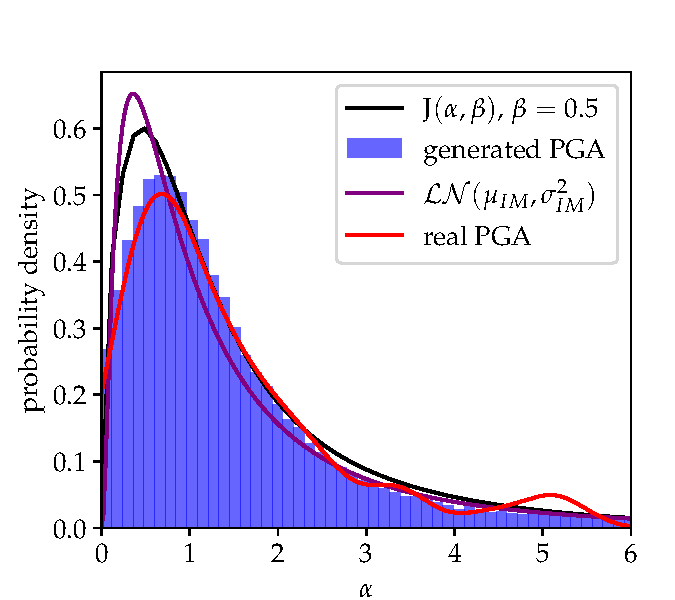
\includegraphics[width=5cm]{figures/uncIM/PGA_density.pdf}}
        {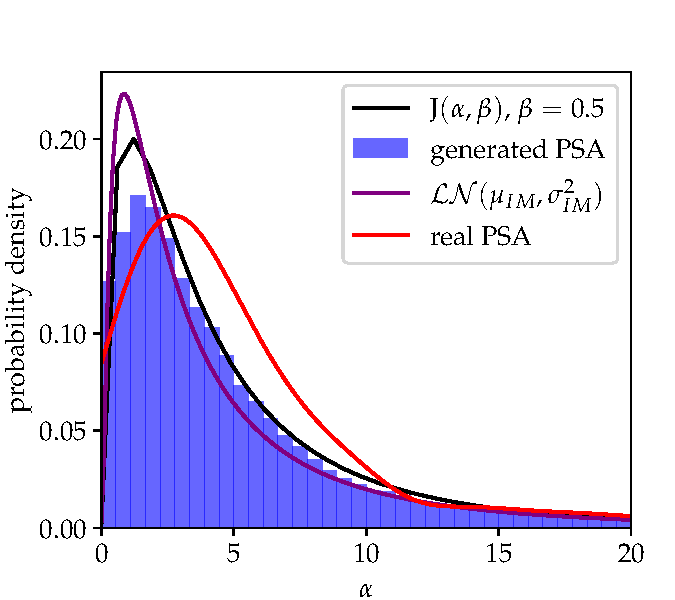
\includegraphics[width=5cm]{figures/uncIM/PSA_density.pdf}}        
        \caption{Comparison of a sectional view of the Jeffreys prior w.r.t. $\alpha$ (black) with the approximated distributions of real accelerograms via Gaussian kernel estimation (red), the histograms of the generated signals (blue) and the log-normal approximations (purple) for the PGA (left) and for the PSA (right).}
         \label{uncIM:fig:IM}
    \end{figure}

        In practice, due to the use of Markov Chain Monte Carlo (MCMC) methods to sample the \emph{a posteriori} distribution, the prior must be evaluated (up to a multiplicative constant) many times in the calculations. Because of its computational complexity due to the integrals to be computed, we performed evaluations of the prior on an experimental design based on a fine-mesh grid of $\Theta$ (here $(0,+\infty)^2$) and to build an interpolated approximation of the Jeffreys prior from this design. This strategy is more suitable for our numerical applications and very tractable because the domain $\Theta$ is only two-dimensional. \Cref{uncIM:fig:jeff_prior} shows plots of the Jeffreys priors. 
%To be precise, $500\times500$ prior values have been computed for $\alpha\in[10^{-5},10]$ and $\beta\in[10^{-3},2]$. A linear interpolation has been processed from these.
        
        \begin{figure}[!ht]
            \centering
            {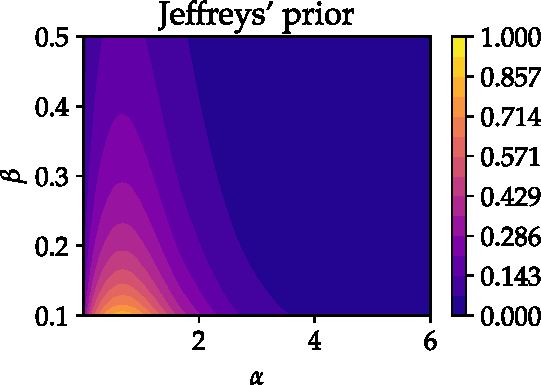
\includegraphics[width=5cm]{figures/PREM/Jeff_prior_PGA-2.pdf}}\hspace*{0.5cm}
            {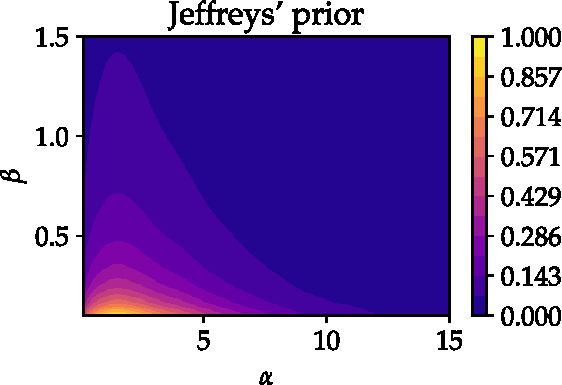
\includegraphics[width=5cm]{figures/PREM/Jeff_prior_PSA-1.pdf}}
            % [PGA]{\includegraphics[width=6cm]{figures/uncIM/Jeff_.pdf}}
            % [PSA]{\includegraphics[width=6cm]{figures/uncIM/Jeffreys_SA.pdf}}
            \caption{The Jeffreys priors calculated from PGA (left) and PSA (right) on subdomains of $\Theta=(0,+\infty)^2$.}
             \label{uncIM:fig:jeff_prior}
        \end{figure}

\section{Estimation tools, competing approaches and benchmarking metrics} \label{uncIM:sec:tools}

    In this section, we first present the Bayesian estimation tools and the Monte-Carlo reference method to which we refer to evaluate the relevance of the log-normal model. Then, to evaluate the performance of the Jeffreys prior, we present two competing approaches that we implement. On the one hand, we apply the MLE method widely used in literature, coupled with a bootstrap technique. On the other hand, we apply a Bayesian technique implemented with the prior introduced by \citet{straub_improved_2008}. Performance evaluation metrics are then defined.

    \subsection{Fragility curves estimations via Monte-Carlo}
     \label{uncIM:sec:reference}
        We assume that a validation data-set $(\mbf a^{\mathrm{MC}},$ $\mbf z^{\mathrm{MC}})$ $ =$ $ ( (a_i^{\mathrm{MC}})_{i=1}^{N^{\mathrm{MC}}} $, $(z_i^{\mathrm{MC}})_{i=1}^{N^{\mathrm{MC}}})$ is available. For nonparametric estimations, good candidates are Monte-Carlo (MC) estimators which estimate the expected number of failures locally w.r.t. the IM. We first need to define a subdivision of the IM values and to estimate the failure probability on each of the sub-intervals. Regular subdivisions are not appropriate because the observed IMs are not uniformly distributed. We follow the suggestion by \citet{trevlopoulos_parametric_2019} to take clusters of the IM using K-means. 
        Given such $N_c$ clusters $(K_j)_{j=1}^{N_c}$, the Monte-Carlo fragility curve estimated at the centroids $(c_j)_{j=1}^{N_c}$ is expressed as
            \begin{equation} \label{uncIM:eq:refMC}
                P_f^{\mathrm{MC}}(c_j) = \frac{1}{n_j}\sum_{i,\,a_i^{\mathrm{MC}}\in K_j}z_i^{\mathrm{MC}}  , 
            \end{equation}
        where $n_j = {\rm Card}(i,\,a_i^{\mathrm{MC}}\in K_j)$ is the size of cluster $K_j$.
        An asymptotic confidence interval for this estimator can also be derived using its Gaussian approximation. It is accepted that a MC-based fragility curve is a reference curve because it is not based on any assumption.

    \subsection{Fragility curves estimations in the Bayesian framework}  \label{uncIM:sec:BayesFram}
        From \cref{uncIM:eq:posterior} \emph{a posteriori} samples of $\theta$ can be obtained by MCMC methods. We have implemented an adaptive Metropolis-Hastings (M-H) algorithm with Gaussian transition kernel and covariance adaptation \citep{haario_adaptive_2001}. Such an algorithm allows for simulations from a probability density known up a multiplicative constant. The \emph{a posteriori} samples of $\theta$ can be used to define credible intervals for the log-normal estimates of the fragility curves.

    \subsection{Competing approaches for performance evaluation} \label{uncIM:sec:Competing}
    
        %\subsubsection{Multiple MLE by bootstrapping} \label{uncIM:sec:bootstrap}
            {\bf Multiple MLE by bootstrapping.}
            The best known parameter estimation method is the MLE, defined as the maximal argument of the likelihood derived from the observed data:
            \begin{equation} \label{uncIM:eq:MLE}
                \hat\theta^{\mathrm{MLE}}_k = \argmax_{\theta\in\Theta} \ell_k(\mbf z|\mbf a, \theta).
            \end{equation}
            A common method for obtaining a wide range of $\theta$  estimates is to compute multiple MLE by bootstrapping. Denoting the data-set size by $k$, bootstrapping consists in doing $L$ independent draws with replacement of $k$ items within the data-set. Those lead to $L$ different likelihoods from the $k$ initial observations, and so to $L$ values of the estimator which can be averaged. In the context of fragility curves, this method is widespread (see e.g. \cite{shinozuka_statistical_2000,lallemant_statistical_2015,gehl_influence_2015,baker_efficient_2015,wang_influence_2020}). The convergence of the MLE and the relevance of this method is stated in \cite{van_der_vaart_asymptotic_1992}. Nevertheless the bootstrap method is often limited by the irregularity of the results for small values of $k$ (see e.g. \cite{zentner_fragility_2017}). In this context, the $L$ values of $\theta$ are used to define confidence intervals for the log-normal estimates of the fragility curves.
 
        
        %\subsubsection{Prior suggested by \citeauthor{Straub2008} \cite{Straub2008}} \label{uncIM:sec:posterioriSimul}
        {\bf Prior suggested by \citet{straub_improved_2008}.}
        This prior, called SK prior, is defined as the product of a normal distribution for $\ln(\alpha)$ and the improper distribution $1/\beta$ for $\beta$, namely:
                \begin{equation} \label{uncIM:eq:Straubprior}
                    \pi_{SK}(\theta)\propto\frac{1}{\alpha\beta} \exp\Big( -\frac{(\log\alpha-\mu)^2}{2\sigma^2}\Big).
                \end{equation}
        In \cite{straub_improved_2008} the parameters $\mu$ and $\sigma$ of the log-normal distribution are chosen to generate a non-informative prior. For a fair comparison with the approach proposed in this paper, we decided to choose $\mu$ and $\sigma$ being equal to the mean and the standard deviation of the logarithm of the IM, whether the PGA or the PSA. This choice is consistent with the fact that the Jeffreys prior is similar to a log-normal distribution with these parameters (see \cref{uncIM:fig:IM}). The prior $\pi_{SK}(\theta)$ is plotted in \cref{uncIM:fig:Straubprior} for the two IMs.

            \begin{figure}[!ht]
                \centering
                {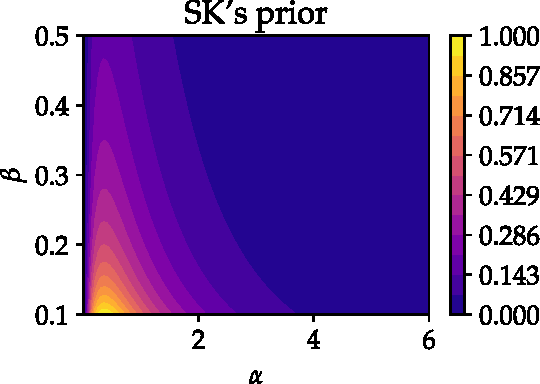
\includegraphics[width=5cm]{figures/PREM/SK_prior_PGA.pdf}}\hspace*{0.5cm}
                {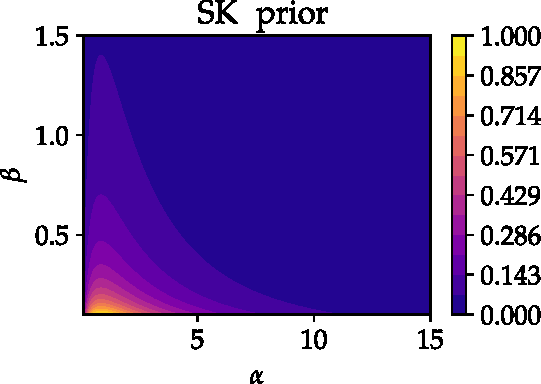
\includegraphics[width=5cm]{figures/PREM/SK_prior_PSA.pdf}}                
                % [PGA]{\includegraphics[width=6cm]{figures/uncIM/SK.pdf}}
                % [PSA]{\includegraphics[width=6cm]{figures/uncIM/SK_prior_SA.pdf}}                
                \caption{Prior suggested by \citet{straub_improved_2008} scaled on log-normal estimations of the PGA (left) and of the PSA (right) distributions.}
                 \label{uncIM:fig:Straubprior}
            \end{figure}

            An analysis of the posterior which results from SK prior is given in \cref{chap:prem}. It shows that the posterior is improper. This statement jeopardizes the validity of \emph{a posteriori} simulations using MCMC methods if we consider the whole domain $\Theta=(0,+\infty)^2$. This issue is nevertheless manageable with the consideration of a truncation w.r.t. $\beta$.
            
            
    \subsection{Benchmarking metrics} \label{uncIM:sec:metrics}
    
        In order to evaluate the performance of the proposed approach, we consider two quantitative metrics which can be calculated for each of the methods described in \cref{uncIM:sec:Competing}.
    We consider the sample $(\mbf a, \mbf z) $. We denote by $a \mapsto P_f^{|\mbf a,\mbf z}(a)$ the random process defined as the fragility curve conditional to the sample (the probability distribution of $P_f^{|\mbf a,\mbf z}(a)$ is inherited from the \emph{a posteriori} distribution of $\theta$). For each value $a$ the $r$-quantile of the random variable $P_f^{|\mbf a,\mbf z}(a)$ is denoted by $q_r^{|\mbf a,\mbf z}(a)$.  
    We define:
    \begin{itemize}
            \item The conditional quadratic error: %{\bf METTRE A JOUR AVEC $\frac{1}{A_{\rm max}}$}
                \begin{equation} \label{uncIM:eq:quaderror}
                \hspace*{-0.3in}
                    \cE^{Q|\mbf a,\mbf z} = \EE\big[\| P_{f}^{|\mbf a,\mbf z} - P_f^{\mathrm{MLE}} \|_{L^2}^2|\mbf a,\mbf z \big] ,\qquad \| P\|_{L^2}^2 = \frac{1}{A_{\rm max}} \int_{0}^{A_{\rm max}} P(a)^2 da .
                \end{equation}
%                \begin{equation} \label{uncIM:eq:quaderror}
%                \hspace*{-0.3in}
%                    \cE^{Q|\mbf a,\mbf z} = \EE\big[\| P_{f}^{|\mbf a,\mbf z} - P_f^{\mathrm{MLE}} \|_{L^2}^2|\mbf a,\mbf z \big] = \int_{0}^{A_{\rm max}} \EE\big[ (P_{f}^{|\mbf a,\mbf z}(a) - P_f^{\mathrm{MLE}} (a))^2 |\mbf a,\mbf z \big] \frac{da}{A_{\rm max}}.
%                \end{equation}
       $P_f^{\mathrm{MLE}}$ stands for the log-normal estimate of the fragility curve obtained by MLE with all the database available. We further check that this estimate is close to the reference curve obtained by MC.             
            \item  The conditional width of the $1-r$ credible zone for the fragility curve:
            %; or the conditional width of the $1-r$ confidence interval for maximum likelihood estimators
                \begin{equation} \label{uncIM:eq:scaleerror}
                    \cS^{r|\mbf a,\mbf z} = \|q_{1-{r/2}}^{|\mbf a,\mbf z} - q_{{r/2}}^{|\mbf a,\mbf z}\|_{L^2}^2  .
                    %= \int_{0}^{A_{\rm max}} ( q_{1-{r/2}}^{|\mbf a,\mbf z} (a) - q_{{r/2}}^{|\mbf a,\mbf z}(a))^2 \frac{da}{A_{\rm max}}  .
                \end{equation}
        \end{itemize}

    To estimate such variables, we simulate a set of $L$ %=5000$ 
    fragility curves $( P_f^{\theta_i|\mbf a,\mbf z})_{i=1}^L$ where $(\theta_i)_{i=1}^L$ is a sample of the \emph{a posteriori} distribution of the model parameters obtained by MCMC. The   empirical quantiles $\hat q_r^{\theta_{i=1}^L|\mbf a,\mbf z}(a)$  of $( P_f^{\theta_i|\mbf a,\mbf z}(a))_{i=1}^L$  are approximations of the quantiles $q_r^{|\mbf a,\mbf z}(a)$ of the random variable $P_f^{|\mbf a,\mbf z}(a)$.
    We derive:
        \begin{itemize}
            \item The approximated conditional quadratic error:
                \begin{equation} \label{uncIM:eq:quaderrorapprox}
                    \hat\cE_{L}^{Q|\mbf a,\mbf z} =\frac{1}{ L}\sum_{i=1}^L\| P_{f}^{\theta_i|\mbf a,\mbf z} - P_f^{\mathrm{MLE}} \|_{L^2}^2.
                \end{equation}
            \item The approximated conditional width of the $1-r$ credible zone for the fragility curve:
                \begin{equation} \label{uncIM:eq:scaleerrorapprox}
                    \hat\cS_L^{r|\mbf a,\mbf z} = \|\hat q_{1-{r/2}}^{\theta_{i=1}^L|\mbf a,\mbf z} - \hat q_{{r/2}}^{\theta_{i=1}^L|\mbf a,\mbf z} \|_{L^2}^2.
                \end{equation}
        \end{itemize}
        The normalized $L^2$ norms are normalized integrals over $a\in [0,A_{\rm max}]$ which are approximated numerically using Simpson's interpolation on a regular subdivision $0=A_0<\dots<A_p=A_{\rm max}$. In the forthcoming section we use   $A_0=0$, $A_{\rm max}=24\,\mathrm{m/s^2}$ for the PGA and $A_{\rm max}=50\,\mathrm{m/s^2}$ for the PSA with $p=200$.

        For the MLE with bootstrapping, we can define a conditional quadratic error as in \cref{uncIM:eq:quaderrorapprox} and conditional width of the $1-r$ confidence interval as in \cref{uncIM:eq:scaleerrorapprox} using a bootstrapped sample $(\theta_i)_{i=1}^L$.


\section{Numerical application} \label{uncIM:sec:application}

\subsection{Presentation of the piping system}

This case study concerns a piping system that is a part of a secondary line of a French Pressurized Water Reactor. This piping system was studied, experimentally and numerically, as part of the ASG program \citep{touboul_seismic_1999}.  \Cref{uncIM:fig:ASG} shows a view of the mock-up mounted on the shaking table Azalee of the EMSI laboratory of CEA/Saclay whereas the Finite Element Model (FEM) ---based on beam elements--- is shown in \cref{uncIM:fig:ASG}-right. The latter has been implemented with the homemade FE code CAST3M~\citep{cea_cast3m_2019} and has been validated via  an experimental campaign.%seismic tests.

	\begin{figure*}[!ht]
		\centering		
		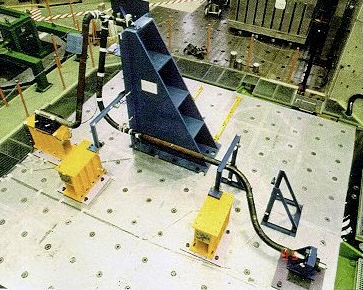
\includegraphics[width=5.2cm]{figures/intro-frags/ASG.jpg}
		\hspace{1cm}
		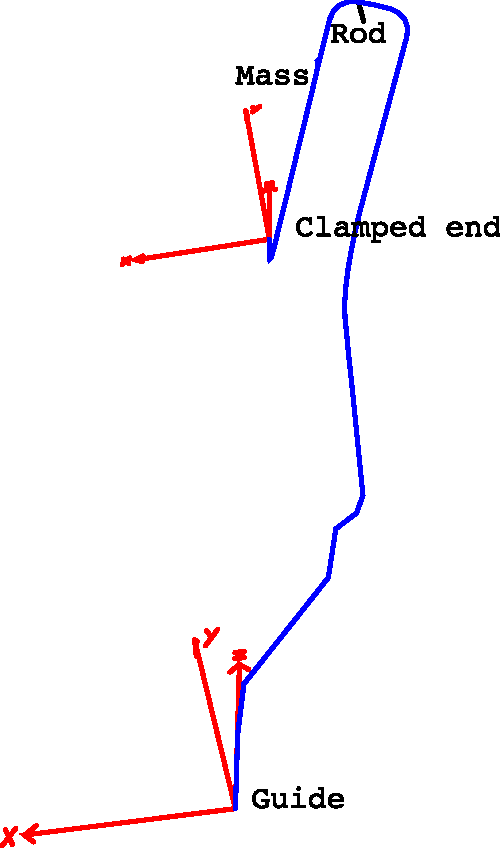
\includegraphics[width=2.5cm]{figures/intro-frags/ASG_FEM.pdf}
		\caption{(left) Overview of the piping system on the Azalee shaking table and (right) Mock-up FEM.}
		 \label{uncIM:fig:ASG}
	\end{figure*}

One end of the mock-up is clamped whereas the other is supported by a guide in order to prevent the displacements in the X and Y directions. Additionally, a rod is  placed on the top of the specimen to limit the mass displacements in the Z direction (see \cref{uncIM:fig:ASG}-right). In the tests, the excitation is only imposed in the X direction. For this study, the artificial signals are filtered by a fictitious $2\%$ damped linear single-mode building at $5$ Hz, the first eigenfrequency of the $1\%$ damped piping system. As failure criterion, we consider excessive out-of-plane rotation of the elbow located near the clamped end of the mock-up, as recommended in \cite{touboul_enhanced_2006}. The critical rotation considered here is equal to $1.6^{\circ}$. This is the level quantile $90\%$ of a sample of size $10^5$ of numerical simulations carried out assuming a linear behavior of the piping system. A linear behavior is considered to simply highlight the influence of the choice of IM. Indeed we use on the one hand the PGA and on the other hand the PSA of the initial set of synthetic signals (i.e not filtered signals), calculated at 5 Hz and 1\% damping ratio. \Cref{uncIM:fig:scatterplots_PSA_PGA} shows that the PSA is clearly better correlated with the response of the structure than the PGA. 

    \begin{figure}[!ht]
        \centering
         {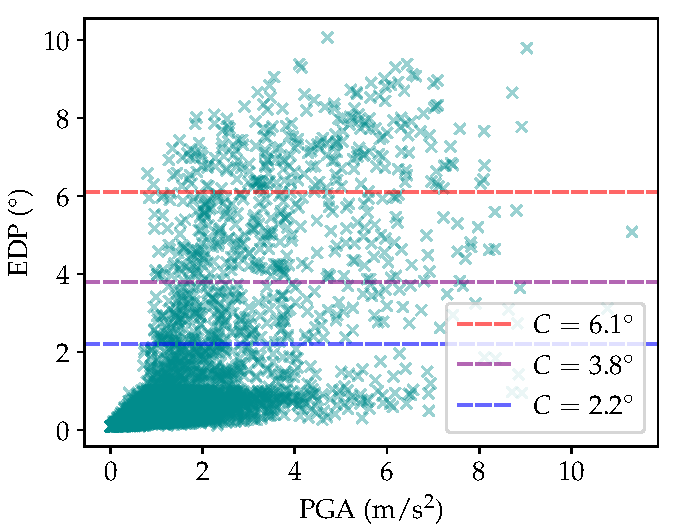
\includegraphics[width=5cm]{figures/uncIM/cloud_PGA.pdf}}
         {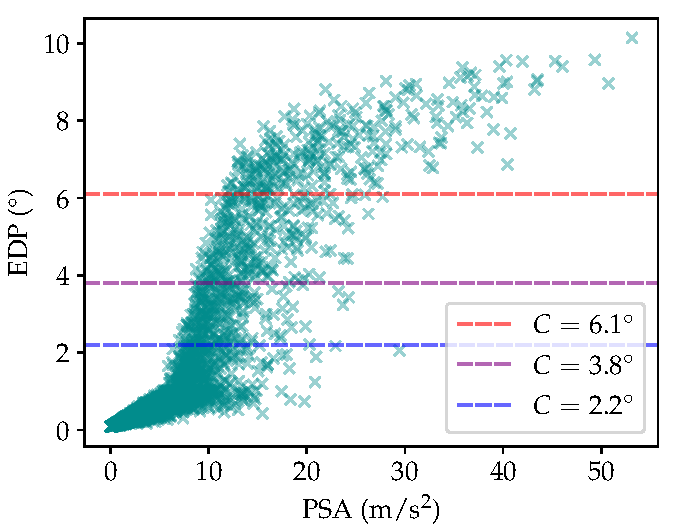
\includegraphics[width=5cm]{figures/uncIM/cloud_PSA.pdf}}
        \caption{Scatter plots of the out-of-plane elbow rotation as a function of (left) PGA and (right) PSA for a linear seismic behavior of the piping system.}
         \label{uncIM:fig:scatterplots_PSA_PGA}
    \end{figure}
    
    For the two IMs, \cref{uncIM:fig:ref-ASG} shows the comparisons between the reference MC-based fragility curves $P_f^{\mathrm{MC}}$ and their log-normal estimates $P_f^{\mathrm{MLE}}$, both estimated via $10^5$ simulations results. In both cases, the log-normal fragility curves are good approximations of the reference ones.

    \begin{figure}[!ht]
        \centering
         {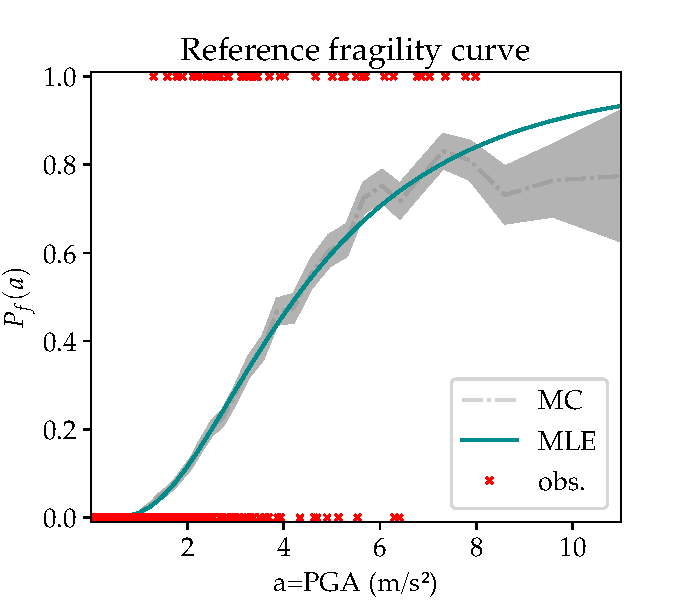
\includegraphics[width=5cm]{figures/uncIM/ref_ASG_PGA.pdf}}
         {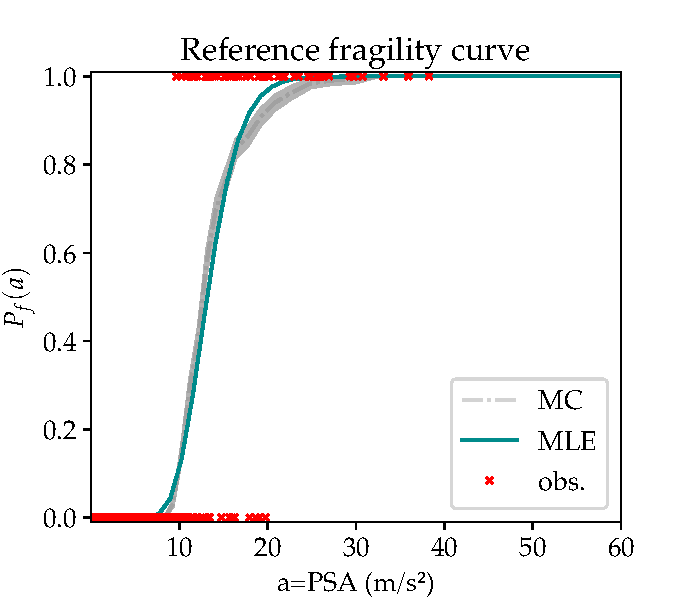
\includegraphics[width=5cm]{figures/uncIM/ref_ASG_PSA.pdf}}
        \caption{Reference fragility curves $P_f^{\mathrm{MC}}$ compared with $P_f^{\mathrm{MLE}}$ computed using the full data-set generated ($10^5$ items) for the PGA (left) and for the PSA (right). The red crosses represent the observations.}
         \label{uncIM:fig:ref-ASG}
    \end{figure}
    
\subsection{Results and discussion}    
    
   \Cref{uncIM:fig:ASG-curves-PGA,uncIM:fig:ASG-curves-SA} present the results for the PGA and the PSA as IM respectively. \nameCrefs{uncIM:fig:ASG-curves-PGA}~\ref{uncIM:fig:ASG-curves-PGA}-(a) and (b) (resp. \namecrefs{uncIM:fig:ASG-curves-SA}~\ref{uncIM:fig:ASG-curves-SA}-(a) and (b)) show the metrics  $\hat\cE_{L,R}^{Q|\mbf a^{(j)},\mbf z^{(j)}}$, $\hat\cS_{L,R}^{r|\mbf a^{(j)},\mbf z^{(j)}}$, $j\in\{1,\dots,m\}$, $R\in\{$`MLE', `SK', `Jeffreys$\}$, $L=5000$, $1-r=95\%$ for any $k$ varying from $15$ to $100$ and $m=200$. \nameCrefs{uncIM:fig:ASG-curves-PGA}~\ref{uncIM:fig:ASG-curves-PGA}-(c) and \ref{uncIM:fig:ASG-curves-SA}-(c) present examples of fragility curves credibility (or confidence for the MLE) intervals for the three methods introduced in \cref{uncIM:sec:Competing} for $k = 30$, in comparison with $P_f^{\mathrm{MLE}}$. 
   Those are computed from generated pairs $(\alpha,\beta)$ whose scatter plots are presented in \namecrefs{uncIM:fig:ASG-curves-PGA}~\ref{uncIM:fig:ASG-curves-PGA}-(d) and \ref{uncIM:fig:ASG-curves-SA}-(d).
   %Finally, figures~\cref{uncIM:fig:ASG-curves-PGA}-(d) and \cref{uncIM:fig:ASG-curves-SA}-(d) present examples of scatter plots of the pair $(\alpha , \beta)$ generated with the three methods.
   
   In addition, to get a better overview on the results, we also show in \cref{uncIM:fig:ASG_CoV} the coefficients of variation of the two parameters $(\alpha , \beta)$ as a function of both IM and $k$.
   
   Generally speaking, these results show, as expected, that when the IM is more correlated to structural response, the differences between the methods are less marked, although in detail there may be some small differences depending on the sample size. {\Cref{uncIM:fig:ASG_CoV} clearly shows that an IM more correlated to the response of the structure induces a lower variability of the estimate of the median of the log-normal model. This is not the case for the log standard deviation whose estimate is affected by samples which are more degenerate with this kind of IM, namely which are partitioned into two disjoint subsets when classified according to IM values: the subset for which there is no failure and the other one for which there is failure, these two subsets possibly being present in the same sample or separately. Such degeneracy affects all methods to varying degrees but in all cases, the Jeffreys prior outperforms SK prior and MLE.}
   
  Whereas the SK prior is calibrated to look like the Jeffreys prior, \namecrefs{uncIM:fig:ASG-curves-PGA}~\ref{uncIM:fig:ASG-curves-PGA}-(d) and \ref{uncIM:fig:ASG-curves-SA}-(d) show that many outliers ---i.e., large values of the pair ($\alpha,\beta$)--- are simulated with the SK prior. These values explain that the credible intervals of the fragility curves and the metrics $\hat\cE_{L,R}^{Q|\mbf a^{(j)},\mbf z^{(j)}}$ and $\hat\cS_{L,R}^{r|\mbf a^{(j)},\mbf z^{(j)}}$ are larger with the SK prior. This observation is both supported by \cref{uncIM:fig:ASG_CoV} and by the calculations provided in \cref{chap:prem} regarding $\beta$. Indeed, in \cref{chap:prem} is shown a better convergence of the Jeffreys prior toward $0$ when $\beta\to\infty$. This better  asymptotic behavior results in posteriors which happen to give a lower probability to outlier points  ---phenomenon particularly noticeable when the data-set is small--- as well as to the weight of the likelihood within the posterior.
  
  Although the intervals compared ---that of the Bayesian framework and that of the MLE--- are not of the same nature ---credible interval for the first \emph{versus} confidence interval for the second--- these results clearly illustrate the advantage of the Bayesian framework over the MLE for small samples. Indeed, irregularities appear in the MLE method that are characterized by null estimates of $\beta$, which result (i) in important coefficient of variation of $\beta$  (\cref{uncIM:fig:ASG_CoV}) and (ii) in ``vertical" confidence intervals on fragility curves estimations (\namecrefs{uncIM:fig:ASG-curves-PGA}~\ref{uncIM:fig:ASG-curves-PGA}-(c) and \ref{uncIM:fig:ASG-curves-SA}-(c)). {When few failures are observed, some samples ---both initial and bootstrapped samples--- are degenerate, as explained earlier.} As no prior is considered in MLE, the likelihood can then be easily maximized with $\beta=0$. In \cref{chap:prem}, it is proven that such scenarios result in degenerate likelihood. This last statement is perceived better through \namecrefs{uncIM:fig:ASG-curves-PGA}~\ref{uncIM:fig:ASG-curves-PGA}-(d) and \ref{uncIM:fig:ASG-curves-SA}-(d). The zero-degenerate $\beta$ values that result from the MLE appear clearly. This leads to a confidence interval generally larger than the credible intervals, except for very small values of $k$ ($k \simeq 20$) when the IM is well correlated with the response of the structure, i.e. with the PSA. Indeed, with a perfect IM - which only exists if we know the structural response itself - the fragility curve is degenerate and has the form of a unit step function. The associated confidence interval is of null size, since in this case it does not require any sample to estimate the fragility curve. So, although apparently better, such confidence intervals are meaningless since they are based on degenerate estimates.
  

  
%\newpage 
          
    \begin{figure}[h]
        \centering
        {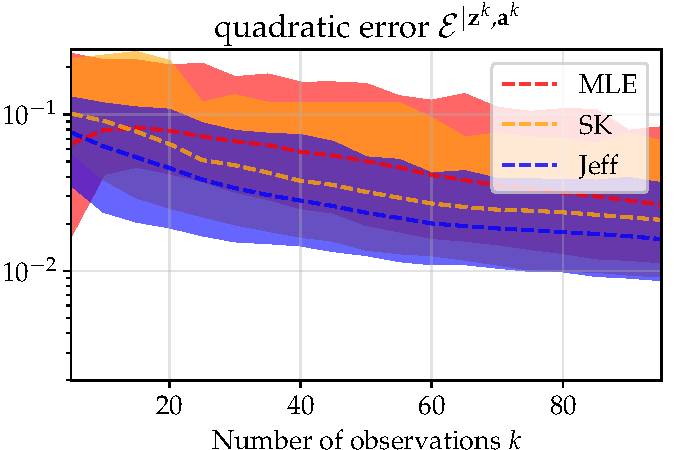
\includegraphics[width=5cm]{figures/uncIM/err_quadra_ASG_PGA.pdf}}\ %
        {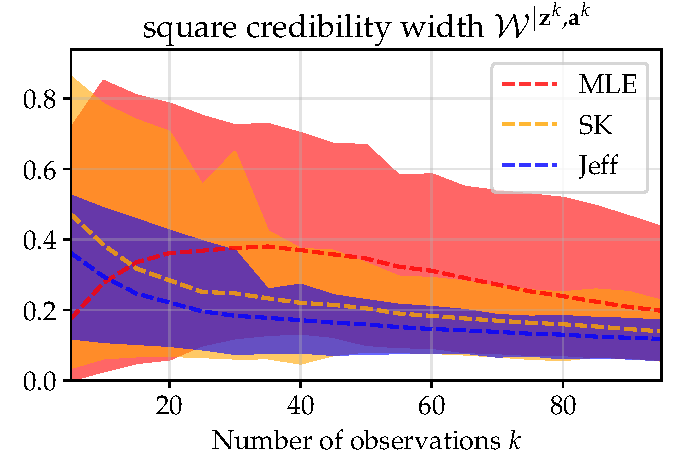
\includegraphics[width=5cm]{figures/uncIM/err_cred_ASG_PGA.pdf}} \\
        \makebox[5cm]{(a)}\ \makebox[5cm]{(b)}\\
        {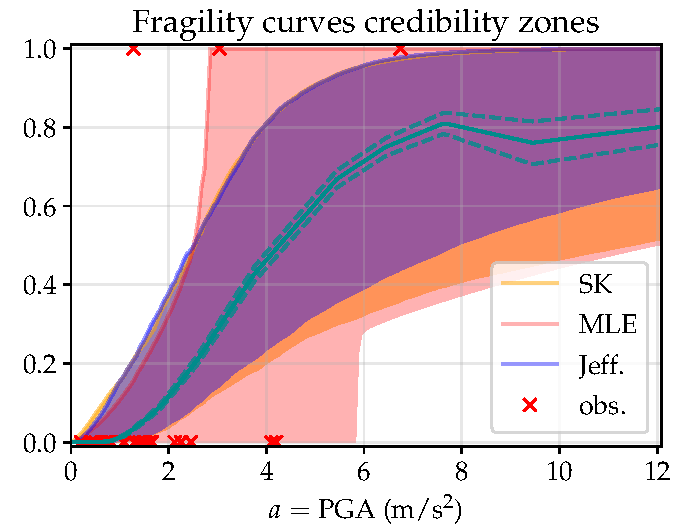
\includegraphics[width=5cm]{figures/uncIM/curves_ASG_PGA.pdf}}\ %           
        {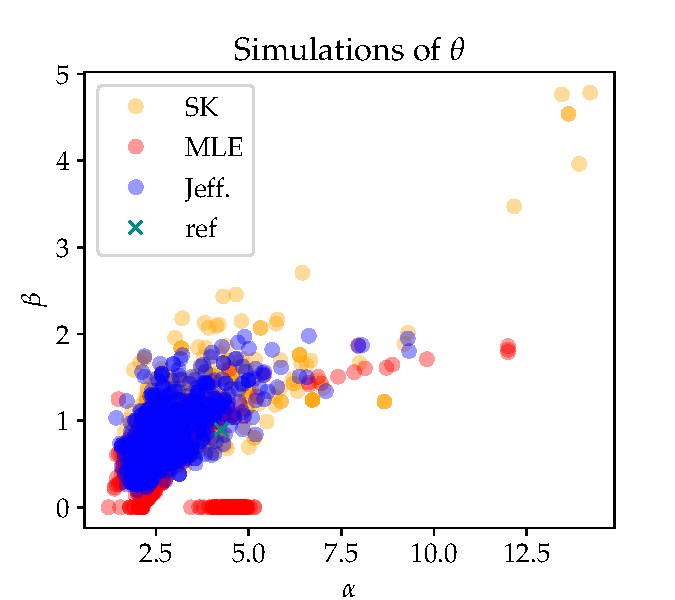
\includegraphics[width=5cm]{figures/uncIM/scatter_ASG_PGA.pdf}}\\
        \makebox[5cm]{(c)}\ \makebox[5cm]{(d)}
         \caption{(a) the dashed lines plot the quadratic errors as a function of the number of data $k$ and the shaded areas show their confidence intervals; (b) the dashed lines plot the widths of the $95\%$ credible intervals (for Bayesian estimation) or confidence intervals (for MLE) and the shaded areas show their confidence intervals; (c) %the dashed lines plot the fragility curve estimates and 
         the shaded areas show the $95\%$ credible (for Bayesian estimation) or confidence (for MLE) intervals resulting from a total of $5000$ simulations of $\theta$ using the three methods considered for $k = 30$; (d) scatter plots of the generated $\theta$ to estimate the fragility curves for the three methods ($500$ points from the $5000$ $\theta=(\alpha,\beta)$ generated are plotted); the green cross in (d) plot $\theta^{\mathrm{MLE}}$ which is used for the computation of $P_f^{\mathrm{MLE}}$, plotted as a green dashed line in (c). Here the PGA is used as IM.}
           \label{uncIM:fig:ASG-curves-PGA}
    \end{figure}

%\newpage             
        
    \begin{figure}[!ht]
        \centering
        {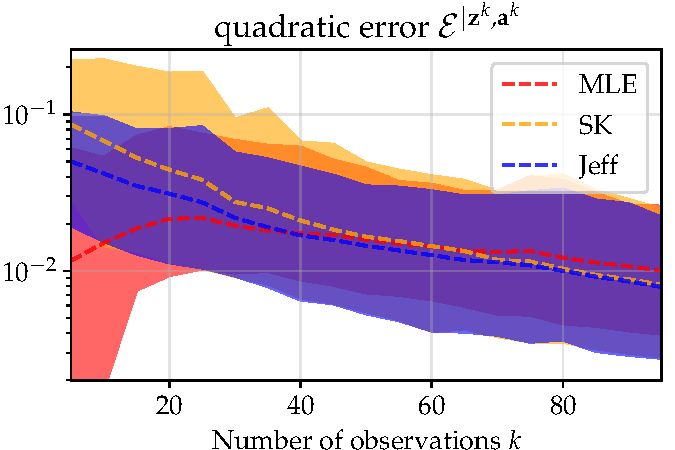
\includegraphics[width=5cm]{figures/uncIM/err_quadra_ASG_PSA.pdf}}\ %
        {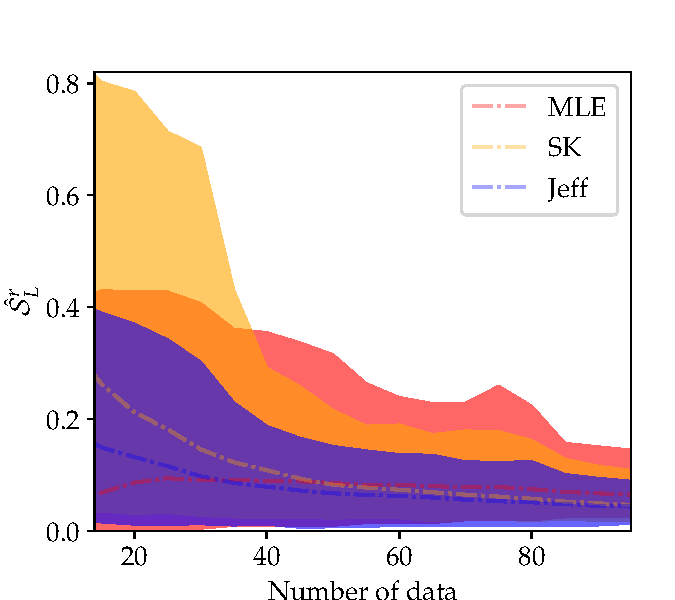
\includegraphics[width=5cm]{figures/uncIM/err_cred_ASG_PSA.pdf}} \\
        \makebox[5cm]{(a)}\ \makebox[5cm]{(b)}\\
        {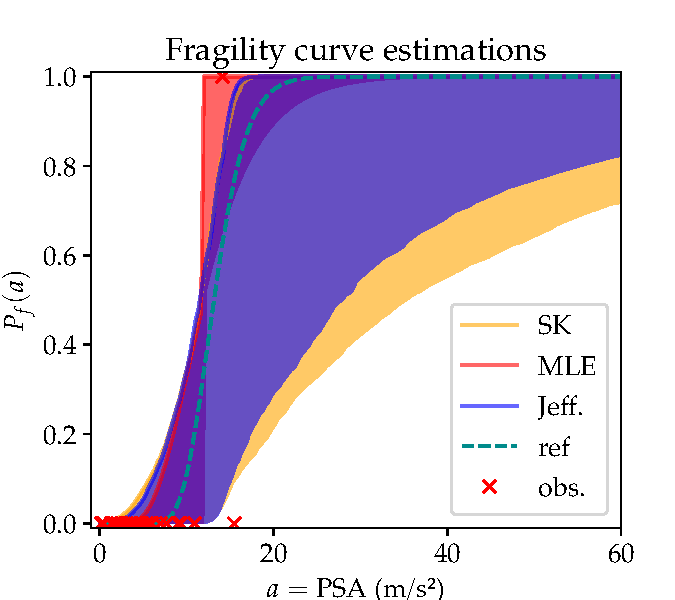
\includegraphics[width=5cm]{figures/uncIM/curves_ASG_PSA.pdf}}\ %           
         {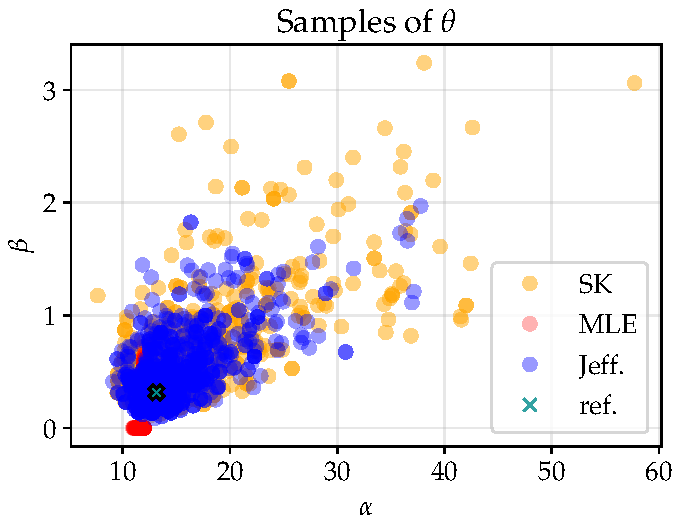
\includegraphics[width=5cm]{figures/uncIM/scatter_ASG_PSA.pdf}}\\
         \makebox[5cm]{(c)}\ \makebox[5cm]{(d)}\\
         \caption{Same as in \cref{uncIM:fig:ASG-curves-PGA}, but here the PSA is used as IM.}
           \label{uncIM:fig:ASG-curves-SA}
    \end{figure}


    As proven in \cref{chap:prem}, in the Bayesian context, the same degenerate samples also produce degeneracy but ``less marked" than for MLE, as the phenomena is regularized by the prior distribution. %, consequently to the regularity brought by the prior. 
    As the results show, this affects SK prior more than Jeffreys one. This is observed, in particular, when the IM is very well correlated with the response of the structure since, in this case, it is more probable to obtain this kind of degenerate samples. Therefore, when $k < 40$, the credible intervals are slightly larger with the PSA than with the PGA. This is also confirmed by the results shown in \cref{uncIM:fig:ASG_CoV}. So, counter-intuitively, when very few data are available, a less well-specified problem from the point of view of the choice of the IM leads to better convergences of the estimates, because it produces fewer degenerate samples. However, this remains confined to very small sample sizes and therefore cannot be considered representative. Note that, in all cases, the Jeffreys prior outperforms SK prior and MLE.


%\newpage 

    \begin{figure}[!ht]
        \centering
        {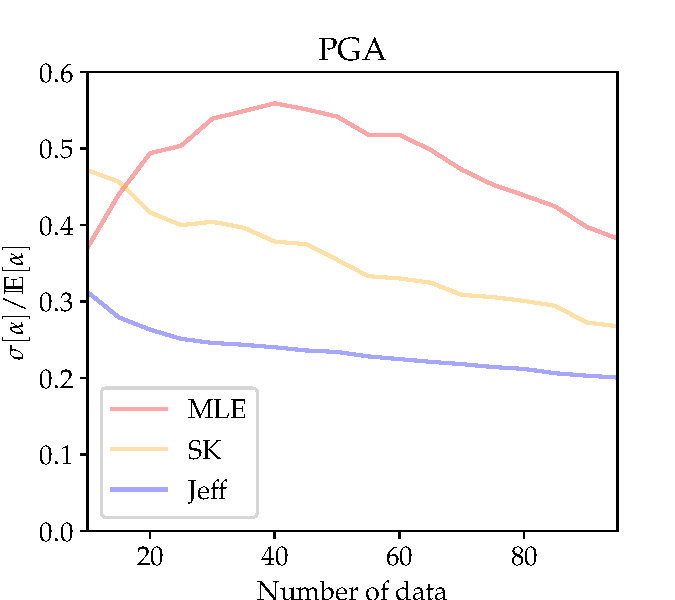
\includegraphics[width=5cm]{figures/uncIM/coeff_alpha_PGA.pdf}}\ %
        {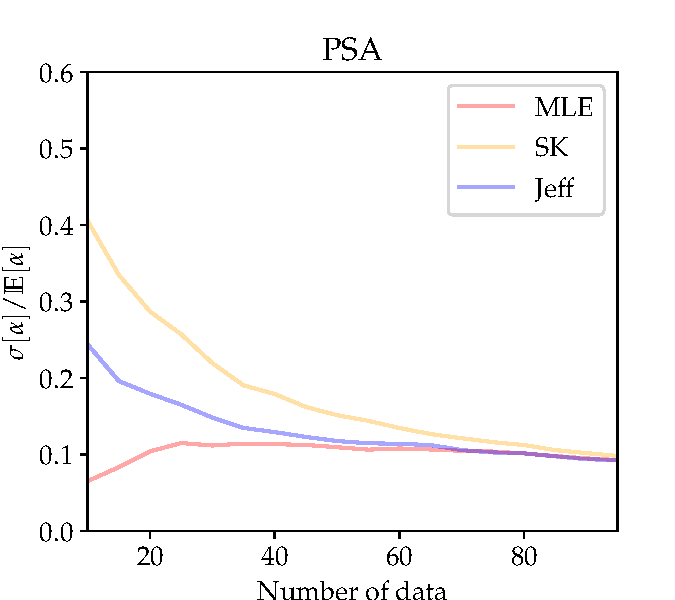
\includegraphics[width=5cm]{figures/uncIM/coeff_alpha_PSA.pdf}} \\
        \makebox[5cm]{(a)}\ \makebox[5cm]{(b)}\\
        {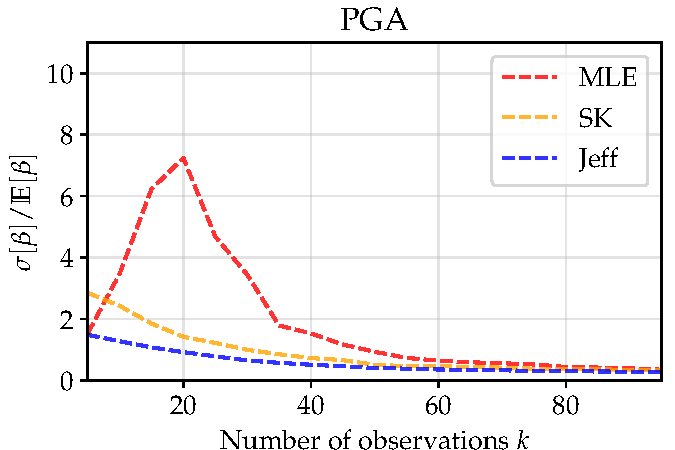
\includegraphics[width=5cm]{figures/uncIM/coeff_beta_PGA.pdf}}\ %           
         {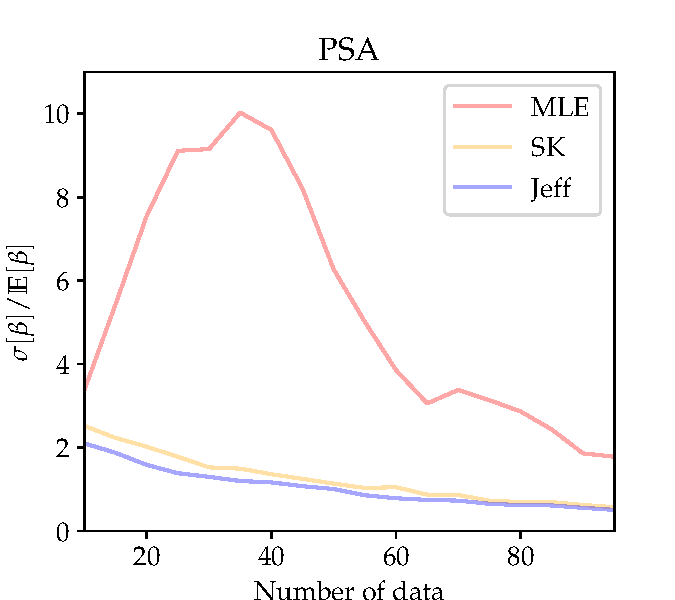
\includegraphics[width=5cm]{figures/uncIM/coeff_beta_PSA.pdf}}\\
         \makebox[5cm]{(c)}\ \makebox[5cm]{(d)}\\
         \caption{Average coefficient of variation of $\alpha$ (a-b) and of $\beta$ (c-d) for the PGA and the PSA. For each value of $k$, $200$ samples of size $k$ have been used to compute the average values of the resulting $200$ coefficients of variation from $5000$ estimates of $\theta$ each.}
           \label{uncIM:fig:ASG_CoV}
    \end{figure}

% \clearpage

\section{Conclusion}  \label{uncIM:sec:conclusion}

Assessing the seismic fragility of Structures and Components when little data is available is a daunting task. The Bayesian framework is known to be efficient for this kind of problems. Nevertheless, the choice of the prior remains tricky because it has a non-negligible influence on the  \emph{a posteriori} distribution and therefore on the estimation of any quantity of interest linked to the fragility curves.

Using the reference prior theory to define an objective prior, we have derived the Jeffreys prior for the log-normal model with binary data which indicate the state of the structure (e.g. failure or non-failure). In doing so, this prior is completely defined, it does not depend on an additional subjective choice.

Since this prior depends only on the characteristics of the ground motion ---the distribution of the IM of interest--- its calculation is then suitable for any equipment of an industrial installation subjected to the same seismic hazard. So, in this work, we were interested in the influence of the choice of the IM ---PGA vs. PSA--- on the convergence of the estimates, for a given (M,R) seismic scenario and a given mechanical structure, namely a piping system.

The results show, as expected, that when the IM is more correlated with the structural response, the differences between methods are less marked, although in detail there may be some small differences depending on sample size, due to possible degenerate samples. {These results testify to the fact that an IM more correlated to the response of the structure essentially induces a lower variability of the estimate of the median of the log-normal model. This is not the case for the log standard deviation whose estimate is affected by samples which are more degenerate with this kind of IM. Such degeneracy affects all methods,} however, in all cases, the Jeffreys prior outperforms the classical approaches of the literature both in terms of regularization (absence of
degenerate estimation) and stability (absence of outliers when sampling the \emph{a posteriori} distribution of the parameters).
